\section{API Service Implementation}
\label{sec:4_9}

The inference API provides real-time fraud scoring, implemented in \texttt{src/api/}.

\subsection{FastAPI Service}
\label{sec:4_9_1}

The FastAPI service exposes a \texttt{POST /predict} endpoint that provides real-time fraud scoring with explanations. The prediction workflow: (1) extracts base features from the incoming event payload using the feature engineering pipeline, (2) enriches features with graph-like statistics by querying the event store for entity-sharing counts (device\_link\_count, ip\_link\_count), (3) generates fraud probability using the trained XGBoost model, (4) computes SHAP values for the prediction to identify top contributing factors, and (5) returns a structured response containing the fraud probability (0-1), categorical risk level (LOW/MEDIUM/HIGH based on thresholds 0.3 and 0.7), and top explanation factors for analyst review. Complete FastAPI implementation with request validation, error handling, and logging is provided in Appendix~A.

\begin{figure}[htbp]
    \centering
    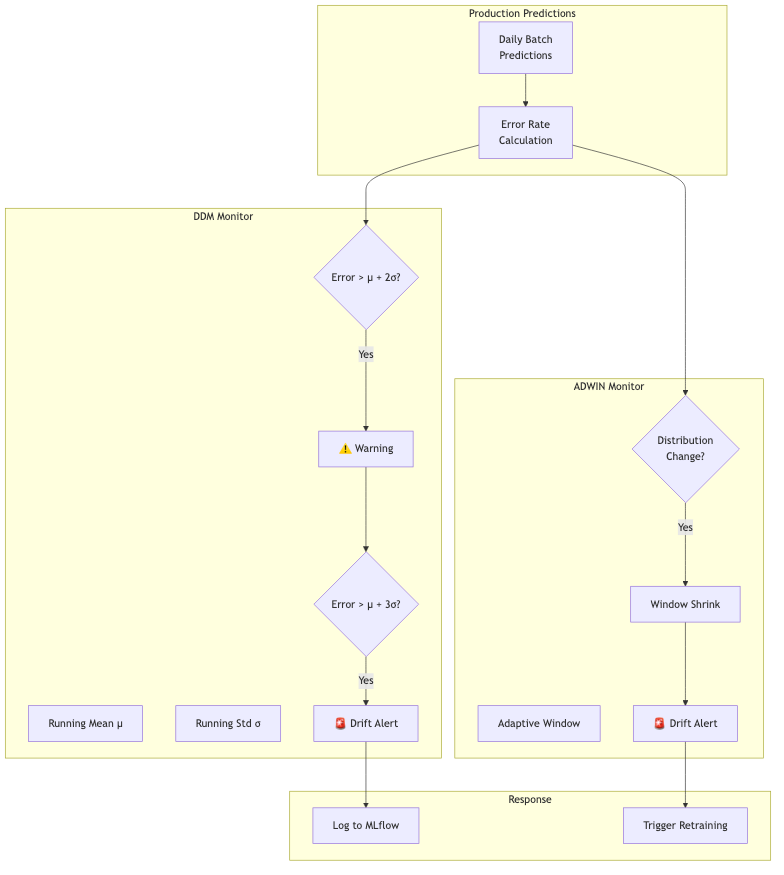
\includegraphics[width=\textwidth]{figures/fig_4_4_7_1.png}
    \caption{API Architecture: FastAPI Service with Event Store}
    \label{fig:4_5}
\end{figure}

\subsection{Event Store}
\label{sec:4_9_2}

The Event Store maintains in-memory storage tracking entity-to-listing mappings for graph-like feature computation without full graph access, enabling low-latency API responses.
